\documentclass[11pt]{article}

    \usepackage[breakable]{tcolorbox}
    \usepackage{parskip} % Stop auto-indenting (to mimic markdown behaviour)
    

    % Basic figure setup, for now with no caption control since it's done
    % automatically by Pandoc (which extracts ![](path) syntax from Markdown).
    \usepackage{graphicx}
    % Keep aspect ratio if custom image width or height is specified
    \setkeys{Gin}{keepaspectratio}
    % Maintain compatibility with old templates. Remove in nbconvert 6.0
    \let\Oldincludegraphics\includegraphics
    % Ensure that by default, figures have no caption (until we provide a
    % proper Figure object with a Caption API and a way to capture that
    % in the conversion process - todo).
    \usepackage{caption}
    \DeclareCaptionFormat{nocaption}{}
    \captionsetup{format=nocaption,aboveskip=0pt,belowskip=0pt}

    \usepackage{float}
    \floatplacement{figure}{H} % forces figures to be placed at the correct location
    \usepackage{xcolor} % Allow colors to be defined
    \usepackage{enumerate} % Needed for markdown enumerations to work
    \usepackage{geometry} % Used to adjust the document margins
    \usepackage{amsmath} % Equations
    \usepackage{amssymb} % Equations
    \usepackage{textcomp} % defines textquotesingle
    % Hack from http://tex.stackexchange.com/a/47451/13684:
    \AtBeginDocument{%
        \def\PYZsq{\textquotesingle}% Upright quotes in Pygmentized code
    }
    \usepackage{upquote} % Upright quotes for verbatim code
    \usepackage{eurosym} % defines \euro

    \usepackage{iftex}
    \ifPDFTeX
        \usepackage[T1]{fontenc}
        \IfFileExists{alphabeta.sty}{
              \usepackage{alphabeta}
          }{
              \usepackage[mathletters]{ucs}
              \usepackage[utf8x]{inputenc}
          }
    \else
        \usepackage{fontspec}
        \usepackage{unicode-math}
    \fi

    \usepackage{fancyvrb} % verbatim replacement that allows latex
    \usepackage{grffile} % extends the file name processing of package graphics
                         % to support a larger range
    \makeatletter % fix for old versions of grffile with XeLaTeX
    \@ifpackagelater{grffile}{2019/11/01}
    {
      % Do nothing on new versions
    }
    {
      \def\Gread@@xetex#1{%
        \IfFileExists{"\Gin@base".bb}%
        {\Gread@eps{\Gin@base.bb}}%
        {\Gread@@xetex@aux#1}%
      }
    }
    \makeatother
    \usepackage[Export]{adjustbox} % Used to constrain images to a maximum size
    \adjustboxset{max size={0.9\linewidth}{0.9\paperheight}}

    % The hyperref package gives us a pdf with properly built
    % internal navigation ('pdf bookmarks' for the table of contents,
    % internal cross-reference links, web links for URLs, etc.)
    \usepackage{hyperref}
    % The default LaTeX title has an obnoxious amount of whitespace. By default,
    % titling removes some of it. It also provides customization options.
    \usepackage{titling}
    \usepackage{longtable} % longtable support required by pandoc >1.10
    \usepackage{booktabs}  % table support for pandoc > 1.12.2
    \usepackage{array}     % table support for pandoc >= 2.11.3
    \usepackage{calc}      % table minipage width calculation for pandoc >= 2.11.1
    \usepackage[inline]{enumitem} % IRkernel/repr support (it uses the enumerate* environment)
    \usepackage[normalem]{ulem} % ulem is needed to support strikethroughs (\sout)
                                % normalem makes italics be italics, not underlines
    \usepackage{soul}      % strikethrough (\st) support for pandoc >= 3.0.0
    \usepackage{mathrsfs}
    

    
    % Colors for the hyperref package
    \definecolor{urlcolor}{rgb}{0,.145,.698}
    \definecolor{linkcolor}{rgb}{.71,0.21,0.01}
    \definecolor{citecolor}{rgb}{.12,.54,.11}

    % ANSI colors
    \definecolor{ansi-black}{HTML}{3E424D}
    \definecolor{ansi-black-intense}{HTML}{282C36}
    \definecolor{ansi-red}{HTML}{E75C58}
    \definecolor{ansi-red-intense}{HTML}{B22B31}
    \definecolor{ansi-green}{HTML}{00A250}
    \definecolor{ansi-green-intense}{HTML}{007427}
    \definecolor{ansi-yellow}{HTML}{DDB62B}
    \definecolor{ansi-yellow-intense}{HTML}{B27D12}
    \definecolor{ansi-blue}{HTML}{208FFB}
    \definecolor{ansi-blue-intense}{HTML}{0065CA}
    \definecolor{ansi-magenta}{HTML}{D160C4}
    \definecolor{ansi-magenta-intense}{HTML}{A03196}
    \definecolor{ansi-cyan}{HTML}{60C6C8}
    \definecolor{ansi-cyan-intense}{HTML}{258F8F}
    \definecolor{ansi-white}{HTML}{C5C1B4}
    \definecolor{ansi-white-intense}{HTML}{A1A6B2}
    \definecolor{ansi-default-inverse-fg}{HTML}{FFFFFF}
    \definecolor{ansi-default-inverse-bg}{HTML}{000000}

    % common color for the border for error outputs.
    \definecolor{outerrorbackground}{HTML}{FFDFDF}

    % commands and environments needed by pandoc snippets
    % extracted from the output of `pandoc -s`
    \providecommand{\tightlist}{%
      \setlength{\itemsep}{0pt}\setlength{\parskip}{0pt}}
    \DefineVerbatimEnvironment{Highlighting}{Verbatim}{commandchars=\\\{\}}
    % Add ',fontsize=\small' for more characters per line
    \newenvironment{Shaded}{}{}
    \newcommand{\KeywordTok}[1]{\textcolor[rgb]{0.00,0.44,0.13}{\textbf{{#1}}}}
    \newcommand{\DataTypeTok}[1]{\textcolor[rgb]{0.56,0.13,0.00}{{#1}}}
    \newcommand{\DecValTok}[1]{\textcolor[rgb]{0.25,0.63,0.44}{{#1}}}
    \newcommand{\BaseNTok}[1]{\textcolor[rgb]{0.25,0.63,0.44}{{#1}}}
    \newcommand{\FloatTok}[1]{\textcolor[rgb]{0.25,0.63,0.44}{{#1}}}
    \newcommand{\CharTok}[1]{\textcolor[rgb]{0.25,0.44,0.63}{{#1}}}
    \newcommand{\StringTok}[1]{\textcolor[rgb]{0.25,0.44,0.63}{{#1}}}
    \newcommand{\CommentTok}[1]{\textcolor[rgb]{0.38,0.63,0.69}{\textit{{#1}}}}
    \newcommand{\OtherTok}[1]{\textcolor[rgb]{0.00,0.44,0.13}{{#1}}}
    \newcommand{\AlertTok}[1]{\textcolor[rgb]{1.00,0.00,0.00}{\textbf{{#1}}}}
    \newcommand{\FunctionTok}[1]{\textcolor[rgb]{0.02,0.16,0.49}{{#1}}}
    \newcommand{\RegionMarkerTok}[1]{{#1}}
    \newcommand{\ErrorTok}[1]{\textcolor[rgb]{1.00,0.00,0.00}{\textbf{{#1}}}}
    \newcommand{\NormalTok}[1]{{#1}}

    % Additional commands for more recent versions of Pandoc
    \newcommand{\ConstantTok}[1]{\textcolor[rgb]{0.53,0.00,0.00}{{#1}}}
    \newcommand{\SpecialCharTok}[1]{\textcolor[rgb]{0.25,0.44,0.63}{{#1}}}
    \newcommand{\VerbatimStringTok}[1]{\textcolor[rgb]{0.25,0.44,0.63}{{#1}}}
    \newcommand{\SpecialStringTok}[1]{\textcolor[rgb]{0.73,0.40,0.53}{{#1}}}
    \newcommand{\ImportTok}[1]{{#1}}
    \newcommand{\DocumentationTok}[1]{\textcolor[rgb]{0.73,0.13,0.13}{\textit{{#1}}}}
    \newcommand{\AnnotationTok}[1]{\textcolor[rgb]{0.38,0.63,0.69}{\textbf{\textit{{#1}}}}}
    \newcommand{\CommentVarTok}[1]{\textcolor[rgb]{0.38,0.63,0.69}{\textbf{\textit{{#1}}}}}
    \newcommand{\VariableTok}[1]{\textcolor[rgb]{0.10,0.09,0.49}{{#1}}}
    \newcommand{\ControlFlowTok}[1]{\textcolor[rgb]{0.00,0.44,0.13}{\textbf{{#1}}}}
    \newcommand{\OperatorTok}[1]{\textcolor[rgb]{0.40,0.40,0.40}{{#1}}}
    \newcommand{\BuiltInTok}[1]{{#1}}
    \newcommand{\ExtensionTok}[1]{{#1}}
    \newcommand{\PreprocessorTok}[1]{\textcolor[rgb]{0.74,0.48,0.00}{{#1}}}
    \newcommand{\AttributeTok}[1]{\textcolor[rgb]{0.49,0.56,0.16}{{#1}}}
    \newcommand{\InformationTok}[1]{\textcolor[rgb]{0.38,0.63,0.69}{\textbf{\textit{{#1}}}}}
    \newcommand{\WarningTok}[1]{\textcolor[rgb]{0.38,0.63,0.69}{\textbf{\textit{{#1}}}}}
    \makeatletter
    \newsavebox\pandoc@box
    \newcommand*\pandocbounded[1]{%
      \sbox\pandoc@box{#1}%
      % scaling factors for width and height
      \Gscale@div\@tempa\textheight{\dimexpr\ht\pandoc@box+\dp\pandoc@box\relax}%
      \Gscale@div\@tempb\linewidth{\wd\pandoc@box}%
      % select the smaller of both
      \ifdim\@tempb\p@<\@tempa\p@
        \let\@tempa\@tempb
      \fi
      % scaling accordingly (\@tempa < 1)
      \ifdim\@tempa\p@<\p@
        \scalebox{\@tempa}{\usebox\pandoc@box}%
      % scaling not needed, use as it is
      \else
        \usebox{\pandoc@box}%
      \fi
    }
    \makeatother

    % Define a nice break command that doesn't care if a line doesn't already
    % exist.
    \def\br{\hspace*{\fill} \\* }
    % Math Jax compatibility definitions
    \def\gt{>}
    \def\lt{<}
    \let\Oldtex\TeX
    \let\Oldlatex\LaTeX
    \renewcommand{\TeX}{\textrm{\Oldtex}}
    \renewcommand{\LaTeX}{\textrm{\Oldlatex}}
    % Document parameters
    % Document title
    \title{GOODChapter3}
    
    
    
    
    
    
    
% Pygments definitions
\makeatletter
\def\PY@reset{\let\PY@it=\relax \let\PY@bf=\relax%
    \let\PY@ul=\relax \let\PY@tc=\relax%
    \let\PY@bc=\relax \let\PY@ff=\relax}
\def\PY@tok#1{\csname PY@tok@#1\endcsname}
\def\PY@toks#1+{\ifx\relax#1\empty\else%
    \PY@tok{#1}\expandafter\PY@toks\fi}
\def\PY@do#1{\PY@bc{\PY@tc{\PY@ul{%
    \PY@it{\PY@bf{\PY@ff{#1}}}}}}}
\def\PY#1#2{\PY@reset\PY@toks#1+\relax+\PY@do{#2}}

\@namedef{PY@tok@w}{\def\PY@tc##1{\textcolor[rgb]{0.73,0.73,0.73}{##1}}}
\@namedef{PY@tok@c}{\let\PY@it=\textit\def\PY@tc##1{\textcolor[rgb]{0.24,0.48,0.48}{##1}}}
\@namedef{PY@tok@cp}{\def\PY@tc##1{\textcolor[rgb]{0.61,0.40,0.00}{##1}}}
\@namedef{PY@tok@k}{\let\PY@bf=\textbf\def\PY@tc##1{\textcolor[rgb]{0.00,0.50,0.00}{##1}}}
\@namedef{PY@tok@kp}{\def\PY@tc##1{\textcolor[rgb]{0.00,0.50,0.00}{##1}}}
\@namedef{PY@tok@kt}{\def\PY@tc##1{\textcolor[rgb]{0.69,0.00,0.25}{##1}}}
\@namedef{PY@tok@o}{\def\PY@tc##1{\textcolor[rgb]{0.40,0.40,0.40}{##1}}}
\@namedef{PY@tok@ow}{\let\PY@bf=\textbf\def\PY@tc##1{\textcolor[rgb]{0.67,0.13,1.00}{##1}}}
\@namedef{PY@tok@nb}{\def\PY@tc##1{\textcolor[rgb]{0.00,0.50,0.00}{##1}}}
\@namedef{PY@tok@nf}{\def\PY@tc##1{\textcolor[rgb]{0.00,0.00,1.00}{##1}}}
\@namedef{PY@tok@nc}{\let\PY@bf=\textbf\def\PY@tc##1{\textcolor[rgb]{0.00,0.00,1.00}{##1}}}
\@namedef{PY@tok@nn}{\let\PY@bf=\textbf\def\PY@tc##1{\textcolor[rgb]{0.00,0.00,1.00}{##1}}}
\@namedef{PY@tok@ne}{\let\PY@bf=\textbf\def\PY@tc##1{\textcolor[rgb]{0.80,0.25,0.22}{##1}}}
\@namedef{PY@tok@nv}{\def\PY@tc##1{\textcolor[rgb]{0.10,0.09,0.49}{##1}}}
\@namedef{PY@tok@no}{\def\PY@tc##1{\textcolor[rgb]{0.53,0.00,0.00}{##1}}}
\@namedef{PY@tok@nl}{\def\PY@tc##1{\textcolor[rgb]{0.46,0.46,0.00}{##1}}}
\@namedef{PY@tok@ni}{\let\PY@bf=\textbf\def\PY@tc##1{\textcolor[rgb]{0.44,0.44,0.44}{##1}}}
\@namedef{PY@tok@na}{\def\PY@tc##1{\textcolor[rgb]{0.41,0.47,0.13}{##1}}}
\@namedef{PY@tok@nt}{\let\PY@bf=\textbf\def\PY@tc##1{\textcolor[rgb]{0.00,0.50,0.00}{##1}}}
\@namedef{PY@tok@nd}{\def\PY@tc##1{\textcolor[rgb]{0.67,0.13,1.00}{##1}}}
\@namedef{PY@tok@s}{\def\PY@tc##1{\textcolor[rgb]{0.73,0.13,0.13}{##1}}}
\@namedef{PY@tok@sd}{\let\PY@it=\textit\def\PY@tc##1{\textcolor[rgb]{0.73,0.13,0.13}{##1}}}
\@namedef{PY@tok@si}{\let\PY@bf=\textbf\def\PY@tc##1{\textcolor[rgb]{0.64,0.35,0.47}{##1}}}
\@namedef{PY@tok@se}{\let\PY@bf=\textbf\def\PY@tc##1{\textcolor[rgb]{0.67,0.36,0.12}{##1}}}
\@namedef{PY@tok@sr}{\def\PY@tc##1{\textcolor[rgb]{0.64,0.35,0.47}{##1}}}
\@namedef{PY@tok@ss}{\def\PY@tc##1{\textcolor[rgb]{0.10,0.09,0.49}{##1}}}
\@namedef{PY@tok@sx}{\def\PY@tc##1{\textcolor[rgb]{0.00,0.50,0.00}{##1}}}
\@namedef{PY@tok@m}{\def\PY@tc##1{\textcolor[rgb]{0.40,0.40,0.40}{##1}}}
\@namedef{PY@tok@gh}{\let\PY@bf=\textbf\def\PY@tc##1{\textcolor[rgb]{0.00,0.00,0.50}{##1}}}
\@namedef{PY@tok@gu}{\let\PY@bf=\textbf\def\PY@tc##1{\textcolor[rgb]{0.50,0.00,0.50}{##1}}}
\@namedef{PY@tok@gd}{\def\PY@tc##1{\textcolor[rgb]{0.63,0.00,0.00}{##1}}}
\@namedef{PY@tok@gi}{\def\PY@tc##1{\textcolor[rgb]{0.00,0.52,0.00}{##1}}}
\@namedef{PY@tok@gr}{\def\PY@tc##1{\textcolor[rgb]{0.89,0.00,0.00}{##1}}}
\@namedef{PY@tok@ge}{\let\PY@it=\textit}
\@namedef{PY@tok@gs}{\let\PY@bf=\textbf}
\@namedef{PY@tok@ges}{\let\PY@bf=\textbf\let\PY@it=\textit}
\@namedef{PY@tok@gp}{\let\PY@bf=\textbf\def\PY@tc##1{\textcolor[rgb]{0.00,0.00,0.50}{##1}}}
\@namedef{PY@tok@go}{\def\PY@tc##1{\textcolor[rgb]{0.44,0.44,0.44}{##1}}}
\@namedef{PY@tok@gt}{\def\PY@tc##1{\textcolor[rgb]{0.00,0.27,0.87}{##1}}}
\@namedef{PY@tok@err}{\def\PY@bc##1{{\setlength{\fboxsep}{\string -\fboxrule}\fcolorbox[rgb]{1.00,0.00,0.00}{1,1,1}{\strut ##1}}}}
\@namedef{PY@tok@kc}{\let\PY@bf=\textbf\def\PY@tc##1{\textcolor[rgb]{0.00,0.50,0.00}{##1}}}
\@namedef{PY@tok@kd}{\let\PY@bf=\textbf\def\PY@tc##1{\textcolor[rgb]{0.00,0.50,0.00}{##1}}}
\@namedef{PY@tok@kn}{\let\PY@bf=\textbf\def\PY@tc##1{\textcolor[rgb]{0.00,0.50,0.00}{##1}}}
\@namedef{PY@tok@kr}{\let\PY@bf=\textbf\def\PY@tc##1{\textcolor[rgb]{0.00,0.50,0.00}{##1}}}
\@namedef{PY@tok@bp}{\def\PY@tc##1{\textcolor[rgb]{0.00,0.50,0.00}{##1}}}
\@namedef{PY@tok@fm}{\def\PY@tc##1{\textcolor[rgb]{0.00,0.00,1.00}{##1}}}
\@namedef{PY@tok@vc}{\def\PY@tc##1{\textcolor[rgb]{0.10,0.09,0.49}{##1}}}
\@namedef{PY@tok@vg}{\def\PY@tc##1{\textcolor[rgb]{0.10,0.09,0.49}{##1}}}
\@namedef{PY@tok@vi}{\def\PY@tc##1{\textcolor[rgb]{0.10,0.09,0.49}{##1}}}
\@namedef{PY@tok@vm}{\def\PY@tc##1{\textcolor[rgb]{0.10,0.09,0.49}{##1}}}
\@namedef{PY@tok@sa}{\def\PY@tc##1{\textcolor[rgb]{0.73,0.13,0.13}{##1}}}
\@namedef{PY@tok@sb}{\def\PY@tc##1{\textcolor[rgb]{0.73,0.13,0.13}{##1}}}
\@namedef{PY@tok@sc}{\def\PY@tc##1{\textcolor[rgb]{0.73,0.13,0.13}{##1}}}
\@namedef{PY@tok@dl}{\def\PY@tc##1{\textcolor[rgb]{0.73,0.13,0.13}{##1}}}
\@namedef{PY@tok@s2}{\def\PY@tc##1{\textcolor[rgb]{0.73,0.13,0.13}{##1}}}
\@namedef{PY@tok@sh}{\def\PY@tc##1{\textcolor[rgb]{0.73,0.13,0.13}{##1}}}
\@namedef{PY@tok@s1}{\def\PY@tc##1{\textcolor[rgb]{0.73,0.13,0.13}{##1}}}
\@namedef{PY@tok@mb}{\def\PY@tc##1{\textcolor[rgb]{0.40,0.40,0.40}{##1}}}
\@namedef{PY@tok@mf}{\def\PY@tc##1{\textcolor[rgb]{0.40,0.40,0.40}{##1}}}
\@namedef{PY@tok@mh}{\def\PY@tc##1{\textcolor[rgb]{0.40,0.40,0.40}{##1}}}
\@namedef{PY@tok@mi}{\def\PY@tc##1{\textcolor[rgb]{0.40,0.40,0.40}{##1}}}
\@namedef{PY@tok@il}{\def\PY@tc##1{\textcolor[rgb]{0.40,0.40,0.40}{##1}}}
\@namedef{PY@tok@mo}{\def\PY@tc##1{\textcolor[rgb]{0.40,0.40,0.40}{##1}}}
\@namedef{PY@tok@ch}{\let\PY@it=\textit\def\PY@tc##1{\textcolor[rgb]{0.24,0.48,0.48}{##1}}}
\@namedef{PY@tok@cm}{\let\PY@it=\textit\def\PY@tc##1{\textcolor[rgb]{0.24,0.48,0.48}{##1}}}
\@namedef{PY@tok@cpf}{\let\PY@it=\textit\def\PY@tc##1{\textcolor[rgb]{0.24,0.48,0.48}{##1}}}
\@namedef{PY@tok@c1}{\let\PY@it=\textit\def\PY@tc##1{\textcolor[rgb]{0.24,0.48,0.48}{##1}}}
\@namedef{PY@tok@cs}{\let\PY@it=\textit\def\PY@tc##1{\textcolor[rgb]{0.24,0.48,0.48}{##1}}}

\def\PYZbs{\char`\\}
\def\PYZus{\char`\_}
\def\PYZob{\char`\{}
\def\PYZcb{\char`\}}
\def\PYZca{\char`\^}
\def\PYZam{\char`\&}
\def\PYZlt{\char`\<}
\def\PYZgt{\char`\>}
\def\PYZsh{\char`\#}
\def\PYZpc{\char`\%}
\def\PYZdl{\char`\$}
\def\PYZhy{\char`\-}
\def\PYZsq{\char`\'}
\def\PYZdq{\char`\"}
\def\PYZti{\char`\~}
% for compatibility with earlier versions
\def\PYZat{@}
\def\PYZlb{[}
\def\PYZrb{]}
\makeatother


    % For linebreaks inside Verbatim environment from package fancyvrb.
    \makeatletter
        \newbox\Wrappedcontinuationbox
        \newbox\Wrappedvisiblespacebox
        \newcommand*\Wrappedvisiblespace {\textcolor{red}{\textvisiblespace}}
        \newcommand*\Wrappedcontinuationsymbol {\textcolor{red}{\llap{\tiny$\m@th\hookrightarrow$}}}
        \newcommand*\Wrappedcontinuationindent {3ex }
        \newcommand*\Wrappedafterbreak {\kern\Wrappedcontinuationindent\copy\Wrappedcontinuationbox}
        % Take advantage of the already applied Pygments mark-up to insert
        % potential linebreaks for TeX processing.
        %        {, <, #, %, $, ' and ": go to next line.
        %        _, }, ^, &, >, - and ~: stay at end of broken line.
        % Use of \textquotesingle for straight quote.
        \newcommand*\Wrappedbreaksatspecials {%
            \def\PYGZus{\discretionary{\char`\_}{\Wrappedafterbreak}{\char`\_}}%
            \def\PYGZob{\discretionary{}{\Wrappedafterbreak\char`\{}{\char`\{}}%
            \def\PYGZcb{\discretionary{\char`\}}{\Wrappedafterbreak}{\char`\}}}%
            \def\PYGZca{\discretionary{\char`\^}{\Wrappedafterbreak}{\char`\^}}%
            \def\PYGZam{\discretionary{\char`\&}{\Wrappedafterbreak}{\char`\&}}%
            \def\PYGZlt{\discretionary{}{\Wrappedafterbreak\char`\<}{\char`\<}}%
            \def\PYGZgt{\discretionary{\char`\>}{\Wrappedafterbreak}{\char`\>}}%
            \def\PYGZsh{\discretionary{}{\Wrappedafterbreak\char`\#}{\char`\#}}%
            \def\PYGZpc{\discretionary{}{\Wrappedafterbreak\char`\%}{\char`\%}}%
            \def\PYGZdl{\discretionary{}{\Wrappedafterbreak\char`\$}{\char`\$}}%
            \def\PYGZhy{\discretionary{\char`\-}{\Wrappedafterbreak}{\char`\-}}%
            \def\PYGZsq{\discretionary{}{\Wrappedafterbreak\textquotesingle}{\textquotesingle}}%
            \def\PYGZdq{\discretionary{}{\Wrappedafterbreak\char`\"}{\char`\"}}%
            \def\PYGZti{\discretionary{\char`\~}{\Wrappedafterbreak}{\char`\~}}%
        }
        % Some characters . , ; ? ! / are not pygmentized.
        % This macro makes them "active" and they will insert potential linebreaks
        \newcommand*\Wrappedbreaksatpunct {%
            \lccode`\~`\.\lowercase{\def~}{\discretionary{\hbox{\char`\.}}{\Wrappedafterbreak}{\hbox{\char`\.}}}%
            \lccode`\~`\,\lowercase{\def~}{\discretionary{\hbox{\char`\,}}{\Wrappedafterbreak}{\hbox{\char`\,}}}%
            \lccode`\~`\;\lowercase{\def~}{\discretionary{\hbox{\char`\;}}{\Wrappedafterbreak}{\hbox{\char`\;}}}%
            \lccode`\~`\:\lowercase{\def~}{\discretionary{\hbox{\char`\:}}{\Wrappedafterbreak}{\hbox{\char`\:}}}%
            \lccode`\~`\?\lowercase{\def~}{\discretionary{\hbox{\char`\?}}{\Wrappedafterbreak}{\hbox{\char`\?}}}%
            \lccode`\~`\!\lowercase{\def~}{\discretionary{\hbox{\char`\!}}{\Wrappedafterbreak}{\hbox{\char`\!}}}%
            \lccode`\~`\/\lowercase{\def~}{\discretionary{\hbox{\char`\/}}{\Wrappedafterbreak}{\hbox{\char`\/}}}%
            \catcode`\.\active
            \catcode`\,\active
            \catcode`\;\active
            \catcode`\:\active
            \catcode`\?\active
            \catcode`\!\active
            \catcode`\/\active
            \lccode`\~`\~
        }
    \makeatother

    \let\OriginalVerbatim=\Verbatim
    \makeatletter
    \renewcommand{\Verbatim}[1][1]{%
        %\parskip\z@skip
        \sbox\Wrappedcontinuationbox {\Wrappedcontinuationsymbol}%
        \sbox\Wrappedvisiblespacebox {\FV@SetupFont\Wrappedvisiblespace}%
        \def\FancyVerbFormatLine ##1{\hsize\linewidth
            \vtop{\raggedright\hyphenpenalty\z@\exhyphenpenalty\z@
                \doublehyphendemerits\z@\finalhyphendemerits\z@
                \strut ##1\strut}%
        }%
        % If the linebreak is at a space, the latter will be displayed as visible
        % space at end of first line, and a continuation symbol starts next line.
        % Stretch/shrink are however usually zero for typewriter font.
        \def\FV@Space {%
            \nobreak\hskip\z@ plus\fontdimen3\font minus\fontdimen4\font
            \discretionary{\copy\Wrappedvisiblespacebox}{\Wrappedafterbreak}
            {\kern\fontdimen2\font}%
        }%

        % Allow breaks at special characters using \PYG... macros.
        \Wrappedbreaksatspecials
        % Breaks at punctuation characters . , ; ? ! and / need catcode=\active
        \OriginalVerbatim[#1,codes*=\Wrappedbreaksatpunct]%
    }
    \makeatother

    % Exact colors from NB
    \definecolor{incolor}{HTML}{303F9F}
    \definecolor{outcolor}{HTML}{D84315}
    \definecolor{cellborder}{HTML}{CFCFCF}
    \definecolor{cellbackground}{HTML}{F7F7F7}

    % prompt
    \makeatletter
    \newcommand{\boxspacing}{\kern\kvtcb@left@rule\kern\kvtcb@boxsep}
    \makeatother
    \newcommand{\prompt}[4]{
        {\ttfamily\llap{{\color{#2}[#3]:\hspace{3pt}#4}}\vspace{-\baselineskip}}
    }
    

    
    % Prevent overflowing lines due to hard-to-break entities
    \sloppy
    % Setup hyperref package
    \hypersetup{
      breaklinks=true,  % so long urls are correctly broken across lines
      colorlinks=true,
      urlcolor=urlcolor,
      linkcolor=linkcolor,
      citecolor=citecolor,
      }
    % Slightly bigger margins than the latex defaults
    
    \geometry{verbose,tmargin=1in,bmargin=1in,lmargin=1in,rmargin=1in}
    
    

\begin{document}
    
    \maketitle
    
    

    
    \section{Chapter 3: Calibration of the HBV
model}\label{chapter-3-calibration-of-the-hbv-model}

    In this chapter the HBV model is calibrated using the observation data.
A set of parameters is used by the HBV model to predict the discharge.
These parameters are optimized using calibration. The model requires
forcings, rainfall and potential evaporation, as inputs. With the
calibrated parameters, it can calculate modelled discharge at the outlet
of the catchment.

The HBV model is available through eWaterCycle. The developer of the
model, Sten Bergström (1992), says the HBV model can best be classified
as a semi-distributed conceptual model. The model consists of three main
components: - subroutines for snow accumulation and melt - subroutines
for soil moisture accounting - response and river routing subroutines

Precipitation and air temperature are the model inputs, and data on
potential evapotranspiration is needed for the accounting of soil
moisture. (Bergström, 1992)

A visual representation of the HBV model can be seen below:

\begin{figure}
\centering
\pandocbounded{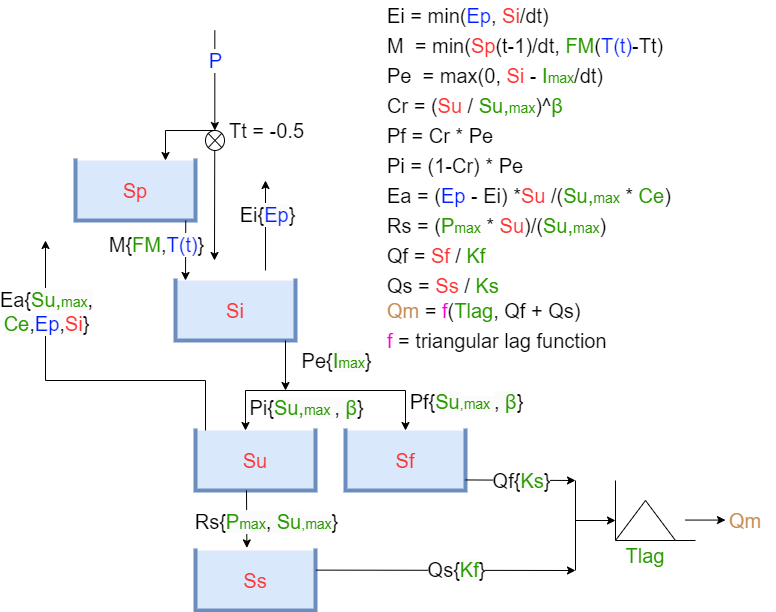
\includegraphics[keepaspectratio]{GOODChapter3_files/77b4b493-6abe-49e9-bb3b-29b3482e5ce8.png}}
\caption{model\_layout.png}
\end{figure}

\emph{Image from the TU Delft course ENVM1502 - ``River Basin
Hydrology'' by Markus Hrachowitz}

    \subsection{General}\label{general}

    First of all, some general python and eWaterCycle libraries need to be
imported:

    \begin{tcolorbox}[breakable, size=fbox, boxrule=1pt, pad at break*=1mm,colback=cellbackground, colframe=cellborder]
\prompt{In}{incolor}{1}{\boxspacing}
\begin{Verbatim}[commandchars=\\\{\}]
\PY{c+c1}{\PYZsh{} general python}
\PY{k+kn}{import}\PY{+w}{ }\PY{n+nn}{warnings}
\PY{n}{warnings}\PY{o}{.}\PY{n}{filterwarnings}\PY{p}{(}\PY{l+s+s2}{\PYZdq{}}\PY{l+s+s2}{ignore}\PY{l+s+s2}{\PYZdq{}}\PY{p}{,} \PY{n}{category}\PY{o}{=}\PY{n+ne}{UserWarning}\PY{p}{)}

\PY{k+kn}{import}\PY{+w}{ }\PY{n+nn}{numpy}\PY{+w}{ }\PY{k}{as}\PY{+w}{ }\PY{n+nn}{np}
\PY{k+kn}{from}\PY{+w}{ }\PY{n+nn}{pathlib}\PY{+w}{ }\PY{k+kn}{import} \PY{n}{Path}
\PY{k+kn}{import}\PY{+w}{ }\PY{n+nn}{pandas}\PY{+w}{ }\PY{k}{as}\PY{+w}{ }\PY{n+nn}{pd}
\PY{k+kn}{import}\PY{+w}{ }\PY{n+nn}{matplotlib}\PY{n+nn}{.}\PY{n+nn}{pyplot}\PY{+w}{ }\PY{k}{as}\PY{+w}{ }\PY{n+nn}{plt}
\PY{k+kn}{import}\PY{+w}{ }\PY{n+nn}{xarray}\PY{+w}{ }\PY{k}{as}\PY{+w}{ }\PY{n+nn}{xr}

\PY{c+c1}{\PYZsh{}niceties}
\PY{k+kn}{from}\PY{+w}{ }\PY{n+nn}{rich}\PY{+w}{ }\PY{k+kn}{import} \PY{n+nb}{print}
\PY{k+kn}{import}\PY{+w}{ }\PY{n+nn}{seaborn}\PY{+w}{ }\PY{k}{as}\PY{+w}{ }\PY{n+nn}{sns}
\PY{n}{sns}\PY{o}{.}\PY{n}{set}\PY{p}{(}\PY{p}{)}

\PY{c+c1}{\PYZsh{}needed}
\PY{k+kn}{from}\PY{+w}{ }\PY{n+nn}{ipywidgets}\PY{+w}{ }\PY{k+kn}{import} \PY{n}{IntProgress}
\PY{k+kn}{from}\PY{+w}{ }\PY{n+nn}{IPython}\PY{n+nn}{.}\PY{n+nn}{display}\PY{+w}{ }\PY{k+kn}{import} \PY{n}{display}

\PY{c+c1}{\PYZsh{} general eWaterCycle}
\PY{k+kn}{import}\PY{+w}{ }\PY{n+nn}{ewatercycle}
\PY{k+kn}{import}\PY{+w}{ }\PY{n+nn}{ewatercycle}\PY{n+nn}{.}\PY{n+nn}{models}
\PY{k+kn}{import}\PY{+w}{ }\PY{n+nn}{ewatercycle}\PY{n+nn}{.}\PY{n+nn}{forcing}
\end{Verbatim}
\end{tcolorbox}

    As stated in chapter 3, eWaterCycle provides access to the Caravan
dataset, from which a Camel dataset of the catchment of the Wien River
is loaded.

    \begin{tcolorbox}[breakable, size=fbox, boxrule=1pt, pad at break*=1mm,colback=cellbackground, colframe=cellborder]
\prompt{In}{incolor}{2}{\boxspacing}
\begin{Verbatim}[commandchars=\\\{\}]
\PY{n}{camelsgb\PYZus{}id} \PY{o}{=} \PY{l+s+s2}{\PYZdq{}}\PY{l+s+s2}{lamah\PYZus{}208082}\PY{l+s+s2}{\PYZdq{}}
\end{Verbatim}
\end{tcolorbox}

    The start and end date of the experiment have to be specified. The start
and end date of the calibration have to be specified as well. The period
of calibration is chosen to be around 75\% of the experiment period.
This means that the model is trained on 75\% of the observation data,
and can be tested on 25\% of the observation data, to make sure the
model is not only working for the data it was trained on, but on other
periods of data as well.

    \begin{tcolorbox}[breakable, size=fbox, boxrule=1pt, pad at break*=1mm,colback=cellbackground, colframe=cellborder]
\prompt{In}{incolor}{3}{\boxspacing}
\begin{Verbatim}[commandchars=\\\{\}]
\PY{c+c1}{\PYZsh{} calibration dates op 75\PYZpc{} van de experiment dates zetten!!!}

\PY{n}{experiment\PYZus{}start\PYZus{}date} \PY{o}{=} \PY{l+s+s2}{\PYZdq{}}\PY{l+s+s2}{1981\PYZhy{}08\PYZhy{}01T00:00:00Z}\PY{l+s+s2}{\PYZdq{}}
\PY{n}{experiment\PYZus{}end\PYZus{}date} \PY{o}{=} \PY{l+s+s2}{\PYZdq{}}\PY{l+s+s2}{2020\PYZhy{}12\PYZhy{}31T00:00:00Z}\PY{l+s+s2}{\PYZdq{}}

\PY{n}{calibration\PYZus{}start\PYZus{}time} \PY{o}{=} \PY{n}{experiment\PYZus{}start\PYZus{}date}
\PY{n}{calibration\PYZus{}end\PYZus{}time} \PY{o}{=} \PY{l+s+s2}{\PYZdq{}}\PY{l+s+s2}{2010\PYZhy{}08\PYZhy{}31T00:00:00Z}\PY{l+s+s2}{\PYZdq{}}

\PY{n}{validation\PYZus{}start\PYZus{}time} \PY{o}{=} \PY{l+s+s2}{\PYZdq{}}\PY{l+s+s2}{2010\PYZhy{}08\PYZhy{}31T00:00:00Z}\PY{l+s+s2}{\PYZdq{}}
\PY{n}{validation\PYZus{}end\PYZus{}time} \PY{o}{=} \PY{n}{experiment\PYZus{}end\PYZus{}date}
\end{Verbatim}
\end{tcolorbox}

    The forcing data can be generated or previously generated data can be
loaded.

    \begin{tcolorbox}[breakable, size=fbox, boxrule=1pt, pad at break*=1mm,colback=cellbackground, colframe=cellborder]
\prompt{In}{incolor}{4}{\boxspacing}
\begin{Verbatim}[commandchars=\\\{\}]
\PY{c+c1}{\PYZsh{} Even though we don\PYZsq{}t use caravan data as forcing, we still call it forcing}
\PY{c+c1}{\PYZsh{} because it is generated using the forcing module of eWaterCycle}
\PY{n}{forcing\PYZus{}path\PYZus{}caravan} \PY{o}{=} \PY{n}{Path}\PY{o}{.}\PY{n}{home}\PY{p}{(}\PY{p}{)} \PY{o}{/} \PY{l+s+s2}{\PYZdq{}}\PY{l+s+s2}{forcing}\PY{l+s+s2}{\PYZdq{}} \PY{o}{/} \PY{n}{camelsgb\PYZus{}id} \PY{o}{/} \PY{l+s+s2}{\PYZdq{}}\PY{l+s+s2}{caravan}\PY{l+s+s2}{\PYZdq{}}
\PY{n}{forcing\PYZus{}path\PYZus{}caravan}\PY{o}{.}\PY{n}{mkdir}\PY{p}{(}\PY{n}{exist\PYZus{}ok}\PY{o}{=}\PY{k+kc}{True}\PY{p}{,} \PY{n}{parents}\PY{o}{=}\PY{k+kc}{True}\PY{p}{)}

\PY{c+c1}{\PYZsh{} If someone has prepared forcing for you, this path needs to be changed to that location. }
\PY{n}{prepared\PYZus{}forcing\PYZus{}path\PYZus{}caravan\PYZus{}central} \PY{o}{=} \PY{n}{Path}\PY{p}{(}\PY{l+s+s2}{\PYZdq{}}\PY{l+s+s2}{location/of/forcing/data}\PY{l+s+s2}{\PYZdq{}}\PY{p}{)}
\end{Verbatim}
\end{tcolorbox}

    \begin{tcolorbox}[breakable, size=fbox, boxrule=1pt, pad at break*=1mm,colback=cellbackground, colframe=cellborder]
\prompt{In}{incolor}{5}{\boxspacing}
\begin{Verbatim}[commandchars=\\\{\}]
\PY{c+c1}{\PYZsh{} \PYZsh{} option one: generate forcing data}
\PY{c+c1}{\PYZsh{} camelsgb\PYZus{}forcing = ewatercycle.forcing.sources[\PYZsq{}CaravanForcing\PYZsq{}].generate(}
\PY{c+c1}{\PYZsh{}     start\PYZus{}time=experiment\PYZus{}start\PYZus{}date,}
\PY{c+c1}{\PYZsh{}     end\PYZus{}time=experiment\PYZus{}end\PYZus{}date,}
\PY{c+c1}{\PYZsh{}     directory=forcing\PYZus{}path\PYZus{}caravan,}
\PY{c+c1}{\PYZsh{}     basin\PYZus{}id=camelsgb\PYZus{}id,}
\PY{c+c1}{\PYZsh{} )}


\PY{c+c1}{\PYZsh{} option two or three: load data that you or someone else generated previously}
\PY{n}{camelsgb\PYZus{}forcing} \PY{o}{=} \PY{n}{ewatercycle}\PY{o}{.}\PY{n}{forcing}\PY{o}{.}\PY{n}{sources}\PY{p}{[}\PY{l+s+s1}{\PYZsq{}}\PY{l+s+s1}{CaravanForcing}\PY{l+s+s1}{\PYZsq{}}\PY{p}{]}\PY{o}{.}\PY{n}{load}\PY{p}{(}\PY{n}{Path}\PY{p}{(}\PY{l+s+s2}{\PYZdq{}}\PY{l+s+s2}{/home/thirza/forcing/lamah\PYZus{}208082/caravan}\PY{l+s+s2}{\PYZdq{}}\PY{p}{)}\PY{p}{)}

\PY{n+nb}{print}\PY{p}{(}\PY{n}{camelsgb\PYZus{}forcing}\PY{p}{)}
\end{Verbatim}
\end{tcolorbox}

    
    \begin{Verbatim}[commandchars=\\\{\}]
\textcolor{ansi-magenta-intense}{\textbf{CaravanForcing}}\textbf{(}
    \textcolor{ansi-yellow}{start\_time}=\textcolor{ansi-green}{'1981-08-01T00:00:00Z'},
    \textcolor{ansi-yellow}{end\_time}=\textcolor{ansi-green}{'2030-12-31T00:00:00Z'},
    \textcolor{ansi-yellow}{directory}=\textcolor{ansi-magenta-intense}{\textbf{PosixPath}}\textbf{(}\textcolor{ansi-green}{'/home/thirza/forcing/lamah\_208082/caravan'}\textbf{)},
    \textcolor{ansi-yellow}{shape}=\textcolor{ansi-magenta-intense}{\textbf{PosixPath}}\textbf{(}\textcolor{ansi-green}{'/home/thirza/forcing/lamah\_208082/caravan/lamah\_208082.shp'}\textbf{)},
    \textcolor{ansi-yellow}{filenames}=\textbf{\{}
        \textcolor{ansi-green}{'tasmax'}: \textcolor{ansi-green}{'lamah\_208082\_1981-08-01\_2030-12-31\_tasmax.nc'},
        \textcolor{ansi-green}{'tas'}: \textcolor{ansi-green}{'lamah\_208082\_1981-08-01\_2030-12-31\_tas.nc'},
        \textcolor{ansi-green}{'tasmin'}: \textcolor{ansi-green}{'lamah\_208082\_1981-08-01\_2030-12-31\_tasmin.nc'},
        \textcolor{ansi-green}{'Q'}: \textcolor{ansi-green}{'lamah\_208082\_1981-08-01\_2030-12-31\_Q.nc'},
        \textcolor{ansi-green}{'pr'}: \textcolor{ansi-green}{'lamah\_208082\_1981-08-01\_2030-12-31\_pr.nc'},
        \textcolor{ansi-green}{'evspsblpot'}: \textcolor{ansi-green}{'lamah\_208082\_1981-08-01\_2030-12-31\_evspsblpot.nc'}
    \textbf{\}}
\textbf{)}

    \end{Verbatim}

    
    Above, it can be seen that the forcing data contains precipitation,
potential evaporation, discharge and the near-surface temperatures
(tas). For this research, only the discharge data is relevant. The
discharge data is loaded from the forcing below, and is plotted.

    \begin{tcolorbox}[breakable, size=fbox, boxrule=1pt, pad at break*=1mm,colback=cellbackground, colframe=cellborder]
\prompt{In}{incolor}{6}{\boxspacing}
\begin{Verbatim}[commandchars=\\\{\}]
\PY{c+c1}{\PYZsh{}quick plot of the discharge data.}
\PY{n}{ds\PYZus{}forcing} \PY{o}{=} \PY{n}{xr}\PY{o}{.}\PY{n}{open\PYZus{}mfdataset}\PY{p}{(}\PY{p}{[}\PY{n}{camelsgb\PYZus{}forcing}\PY{p}{[}\PY{l+s+s1}{\PYZsq{}}\PY{l+s+s1}{Q}\PY{l+s+s1}{\PYZsq{}}\PY{p}{]}\PY{p}{]}\PY{p}{)}
\PY{n}{ds\PYZus{}forcing}\PY{p}{[}\PY{l+s+s2}{\PYZdq{}}\PY{l+s+s2}{Q}\PY{l+s+s2}{\PYZdq{}}\PY{p}{]}\PY{o}{.}\PY{n}{plot}\PY{p}{(}\PY{p}{)}
\end{Verbatim}
\end{tcolorbox}

            \begin{tcolorbox}[breakable, size=fbox, boxrule=.5pt, pad at break*=1mm, opacityfill=0]
\prompt{Out}{outcolor}{6}{\boxspacing}
\begin{Verbatim}[commandchars=\\\{\}]
[<matplotlib.lines.Line2D at 0x7f26f16205c0>]
\end{Verbatim}
\end{tcolorbox}
        
    \begin{center}
    \adjustimage{max size={0.9\linewidth}{0.9\paperheight}}{GOODChapter3_files/GOODChapter3_13_1.png}
    \end{center}
    { \hspace*{\fill} \\}
    
    \subsection{Calibration}\label{calibration}

    The HBV model contains five stores where the water is stored and nine
parameters that control the flow between those stores and in and out of
the model. For the storages an array of starting values is specified.
The values for the parameters will later be estimated using
optimization.

    \begin{tcolorbox}[breakable, size=fbox, boxrule=1pt, pad at break*=1mm,colback=cellbackground, colframe=cellborder]
\prompt{In}{incolor}{7}{\boxspacing}
\begin{Verbatim}[commandchars=\\\{\}]
\PY{c+c1}{\PYZsh{}               Si,  Su, Sf, Ss, Sp}
\PY{n}{s\PYZus{}0} \PY{o}{=} \PY{n}{np}\PY{o}{.}\PY{n}{array}\PY{p}{(}\PY{p}{[}\PY{l+m+mi}{0}\PY{p}{,}  \PY{l+m+mi}{100}\PY{p}{,}  \PY{l+m+mi}{0}\PY{p}{,}  \PY{l+m+mi}{5}\PY{p}{,} \PY{l+m+mi}{0}\PY{p}{]}\PY{p}{)}
\PY{n}{S\PYZus{}names} \PY{o}{=} \PY{p}{[}\PY{l+s+s2}{\PYZdq{}}\PY{l+s+s2}{Interception storage}\PY{l+s+s2}{\PYZdq{}}\PY{p}{,} \PY{l+s+s2}{\PYZdq{}}\PY{l+s+s2}{Unsaturated Rootzone Storage}\PY{l+s+s2}{\PYZdq{}}\PY{p}{,} \PY{l+s+s2}{\PYZdq{}}\PY{l+s+s2}{Fastflow storage}\PY{l+s+s2}{\PYZdq{}}\PY{p}{,} \PY{l+s+s2}{\PYZdq{}}\PY{l+s+s2}{Slowflow storage}\PY{l+s+s2}{\PYZdq{}}\PY{p}{,} \PY{l+s+s2}{\PYZdq{}}\PY{l+s+s2}{Groundwater storage}\PY{l+s+s2}{\PYZdq{}}\PY{p}{]}

\PY{n}{p\PYZus{}names} \PY{o}{=} \PY{p}{[}\PY{l+s+s2}{\PYZdq{}}\PY{l+s+s2}{\PYZdl{}I\PYZus{}}\PY{l+s+si}{\PYZob{}max\PYZcb{}}\PY{l+s+s2}{\PYZdl{}}\PY{l+s+s2}{\PYZdq{}}\PY{p}{,}  \PY{l+s+s2}{\PYZdq{}}\PY{l+s+s2}{\PYZdl{}C\PYZus{}e\PYZdl{}}\PY{l+s+s2}{\PYZdq{}}\PY{p}{,}  \PY{l+s+s2}{\PYZdq{}}\PY{l+s+s2}{\PYZdl{}Su\PYZus{}}\PY{l+s+si}{\PYZob{}max\PYZcb{}}\PY{l+s+s2}{\PYZdl{}}\PY{l+s+s2}{\PYZdq{}}\PY{p}{,} \PY{l+s+s2}{\PYZdq{}}\PY{l+s+s2}{β}\PY{l+s+s2}{\PYZdq{}}\PY{p}{,}  \PY{l+s+s2}{\PYZdq{}}\PY{l+s+s2}{\PYZdl{}P\PYZus{}}\PY{l+s+si}{\PYZob{}max\PYZcb{}}\PY{l+s+s2}{\PYZdl{}}\PY{l+s+s2}{\PYZdq{}}\PY{p}{,}  \PY{l+s+s2}{\PYZdq{}}\PY{l+s+s2}{\PYZdl{}T\PYZus{}}\PY{l+s+si}{\PYZob{}lag\PYZcb{}}\PY{l+s+s2}{\PYZdl{}}\PY{l+s+s2}{\PYZdq{}}\PY{p}{,}   \PY{l+s+s2}{\PYZdq{}}\PY{l+s+s2}{\PYZdl{}K\PYZus{}f\PYZdl{}}\PY{l+s+s2}{\PYZdq{}}\PY{p}{,}   \PY{l+s+s2}{\PYZdq{}}\PY{l+s+s2}{\PYZdl{}K\PYZus{}s\PYZdl{}}\PY{l+s+s2}{\PYZdq{}}\PY{p}{,} \PY{l+s+s2}{\PYZdq{}}\PY{l+s+s2}{FM}\PY{l+s+s2}{\PYZdq{}}\PY{p}{]}
\PY{n}{param\PYZus{}names} \PY{o}{=} \PY{p}{[}\PY{l+s+s2}{\PYZdq{}}\PY{l+s+s2}{Imax}\PY{l+s+s2}{\PYZdq{}}\PY{p}{,}\PY{l+s+s2}{\PYZdq{}}\PY{l+s+s2}{Ce}\PY{l+s+s2}{\PYZdq{}}\PY{p}{,}  \PY{l+s+s2}{\PYZdq{}}\PY{l+s+s2}{Sumax}\PY{l+s+s2}{\PYZdq{}}\PY{p}{,} \PY{l+s+s2}{\PYZdq{}}\PY{l+s+s2}{beta}\PY{l+s+s2}{\PYZdq{}}\PY{p}{,}  \PY{l+s+s2}{\PYZdq{}}\PY{l+s+s2}{Pmax}\PY{l+s+s2}{\PYZdq{}}\PY{p}{,}  \PY{l+s+s2}{\PYZdq{}}\PY{l+s+s2}{Tlag}\PY{l+s+s2}{\PYZdq{}}\PY{p}{,}   \PY{l+s+s2}{\PYZdq{}}\PY{l+s+s2}{Kf}\PY{l+s+s2}{\PYZdq{}}\PY{p}{,}   \PY{l+s+s2}{\PYZdq{}}\PY{l+s+s2}{Ks}\PY{l+s+s2}{\PYZdq{}}\PY{p}{,} \PY{l+s+s2}{\PYZdq{}}\PY{l+s+s2}{FM}\PY{l+s+s2}{\PYZdq{}}\PY{p}{]}\PYZbs{}

\PY{c+c1}{\PYZsh{} p\PYZus{}min\PYZus{}initial= np.array([0,   0.2,  40,    .5,   .001,   1,     .01,  .0001,  .01])}
\PY{c+c1}{\PYZsh{} p\PYZus{}max\PYZus{}initial = np.array([8,    1,  800,   4,    .3,     10,    .1,   .01,  0.5])}

\PY{c+c1}{\PYZsh{} p\PYZus{}min\PYZus{}initial= np.array([0,   0.2,  40,    .5,   .001,   0.1,  .01,  .0001,  .01])}
\PY{c+c1}{\PYZsh{} p\PYZus{}max\PYZus{}initial = np.array([8,    4,  800,   4,    3,     10,    3,   .1,  5])}
\end{Verbatim}
\end{tcolorbox}

    \subsubsection{Kling Gupta efficiency}\label{kling-gupta-efficiency}

    For my research, the height and frequency of the peaks are important,
but their timing is less critical. The Kling-Gupta Efficiency is a
measure that evaluates how well a model performs by looking at
correlation, bias, and variability. By using an altered Kling-Gupta
Efficiency in which the correlation is being left out, the timing of the
peaks is not being taken into account. This method is useful for
predicting the size of peaks and the overall distribution, while being
less focused on the exact timing of the peaks.

    A good way to predict the best parameter combination is through
Nelder-Mead optimization. This optimization method finds the minimum of
a function. The result of the Nelder-Mead optimization is the best
parameter combination the method found. The Nelder-Mead optimization is
run using the Kling-Gupta efficiency.

    \begin{tcolorbox}[breakable, size=fbox, boxrule=1pt, pad at break*=1mm,colback=cellbackground, colframe=cellborder]
\prompt{In}{incolor}{8}{\boxspacing}
\begin{Verbatim}[commandchars=\\\{\}]
\PY{k+kn}{import}\PY{+w}{ }\PY{n+nn}{numpy}\PY{+w}{ }\PY{k}{as}\PY{+w}{ }\PY{n+nn}{np}
\PY{n}{Q\PYZus{}pandas} \PY{o}{=} \PY{n}{ds\PYZus{}forcing}\PY{p}{[}\PY{l+s+s2}{\PYZdq{}}\PY{l+s+s2}{Q}\PY{l+s+s2}{\PYZdq{}}\PY{p}{]}\PY{o}{.}\PY{n}{to\PYZus{}dataframe}\PY{p}{(}\PY{p}{)}
\PY{k}{def}\PY{+w}{ }\PY{n+nf}{kling\PYZus{}gupta\PYZus{}efficiency}\PY{p}{(}\PY{n}{obs}\PY{p}{,} \PY{n}{sim}\PY{p}{,} \PY{n}{start\PYZus{}calibration}\PY{p}{,} \PY{n}{end\PYZus{}calibration}\PY{p}{)}\PY{p}{:}

    \PY{c+c1}{\PYZsh{}combine the two in one dataFrame}
    \PY{n}{hydro\PYZus{}data} \PY{o}{=} \PY{n}{pd}\PY{o}{.}\PY{n}{concat}\PY{p}{(}\PY{p}{[}\PY{n}{sim}\PY{o}{.}\PY{n}{reindex}\PY{p}{(}\PY{n}{obs}\PY{o}{.}\PY{n}{index}\PY{p}{,} \PY{n}{method} \PY{o}{=} \PY{l+s+s1}{\PYZsq{}}\PY{l+s+s1}{ffill}\PY{l+s+s1}{\PYZsq{}}\PY{p}{)}\PY{p}{,} \PY{n}{obs}\PY{p}{]}\PY{p}{,} \PY{n}{axis}\PY{o}{=}\PY{l+m+mi}{1}\PY{p}{)}

    \PY{c+c1}{\PYZsh{}only select the calibration period}
    \PY{n}{hydro\PYZus{}data} \PY{o}{=} \PY{n}{hydro\PYZus{}data}\PY{p}{[}\PY{n}{hydro\PYZus{}data}\PY{o}{.}\PY{n}{index} \PY{o}{\PYZgt{}} \PY{n}{pd}\PY{o}{.}\PY{n}{to\PYZus{}datetime}\PY{p}{(}\PY{n}{pd}\PY{o}{.}\PY{n}{Timestamp}\PY{p}{(}\PY{n}{start\PYZus{}calibration}\PY{p}{)}\PY{o}{.}\PY{n}{date}\PY{p}{(}\PY{p}{)}\PY{p}{)}\PY{p}{]}
    \PY{n}{hydro\PYZus{}data} \PY{o}{=} \PY{n}{hydro\PYZus{}data}\PY{p}{[}\PY{n}{hydro\PYZus{}data}\PY{o}{.}\PY{n}{index} \PY{o}{\PYZlt{}} \PY{n}{pd}\PY{o}{.}\PY{n}{to\PYZus{}datetime}\PY{p}{(}\PY{n}{pd}\PY{o}{.}\PY{n}{Timestamp}\PY{p}{(}\PY{n}{end\PYZus{}calibration}\PY{p}{)}\PY{o}{.}\PY{n}{date}\PY{p}{(}\PY{p}{)}\PY{p}{)}\PY{p}{]}


    \PY{c+c1}{\PYZsh{}  \PYZsh{}calculate mean absolute difference to the power 4, so peaks weigh more}
    \PY{c+c1}{\PYZsh{} diff = (hydro\PYZus{}data[\PYZsq{}Q\PYZsq{}] \PYZhy{} hydro\PYZus{}data[\PYZsq{}model output\PYZsq{}]) }
    \PY{c+c1}{\PYZsh{} absDiff = np.abs(diff)}
    \PY{c+c1}{\PYZsh{} meanAbsDiff = np.mean(absDiff)}
    
    \PY{n}{r} \PY{o}{=} \PY{n}{np}\PY{o}{.}\PY{n}{corrcoef}\PY{p}{(}\PY{n}{hydro\PYZus{}data}\PY{p}{[}\PY{l+s+s1}{\PYZsq{}}\PY{l+s+s1}{Q}\PY{l+s+s1}{\PYZsq{}}\PY{p}{]}\PY{p}{,} \PY{n}{hydro\PYZus{}data}\PY{p}{[}\PY{l+s+s1}{\PYZsq{}}\PY{l+s+s1}{model output}\PY{l+s+s1}{\PYZsq{}}\PY{p}{]}\PY{p}{)}\PY{p}{[}\PY{l+m+mi}{0}\PY{p}{,} \PY{l+m+mi}{1}\PY{p}{]}  \PY{c+c1}{\PYZsh{} Correlation}
    \PY{n}{beta} \PY{o}{=} \PY{n}{np}\PY{o}{.}\PY{n}{mean}\PY{p}{(}\PY{n}{hydro\PYZus{}data}\PY{p}{[}\PY{l+s+s1}{\PYZsq{}}\PY{l+s+s1}{model output}\PY{l+s+s1}{\PYZsq{}}\PY{p}{]}\PY{p}{)} \PY{o}{/} \PY{n}{np}\PY{o}{.}\PY{n}{mean}\PY{p}{(}\PY{n}{hydro\PYZus{}data}\PY{p}{[}\PY{l+s+s1}{\PYZsq{}}\PY{l+s+s1}{Q}\PY{l+s+s1}{\PYZsq{}}\PY{p}{]}\PY{p}{)}  \PY{c+c1}{\PYZsh{} Bias ratio}
    \PY{n}{gamma} \PY{o}{=} \PY{n}{np}\PY{o}{.}\PY{n}{std}\PY{p}{(}\PY{n}{hydro\PYZus{}data}\PY{p}{[}\PY{l+s+s1}{\PYZsq{}}\PY{l+s+s1}{model output}\PY{l+s+s1}{\PYZsq{}}\PY{p}{]}\PY{p}{)} \PY{o}{/} \PY{n}{np}\PY{o}{.}\PY{n}{std}\PY{p}{(}\PY{n}{hydro\PYZus{}data}\PY{p}{[}\PY{l+s+s1}{\PYZsq{}}\PY{l+s+s1}{Q}\PY{l+s+s1}{\PYZsq{}}\PY{p}{]}\PY{p}{)}  \PY{c+c1}{\PYZsh{} Variability ratio}

    \PY{n}{mean\PYZus{}pieken\PYZus{}output} \PY{o}{=} \PY{n}{hydro\PYZus{}data}\PY{p}{[}\PY{n}{hydro\PYZus{}data}\PY{p}{[}\PY{l+s+s1}{\PYZsq{}}\PY{l+s+s1}{model output}\PY{l+s+s1}{\PYZsq{}}\PY{p}{]} \PY{o}{\PYZgt{}} \PY{n}{hydro\PYZus{}data}\PY{p}{[}\PY{l+s+s1}{\PYZsq{}}\PY{l+s+s1}{model output}\PY{l+s+s1}{\PYZsq{}}\PY{p}{]}\PY{o}{.}\PY{n}{quantile}\PY{p}{(}\PY{l+m+mf}{0.95}\PY{p}{)}\PY{p}{]}\PY{p}{[}\PY{l+s+s2}{\PYZdq{}}\PY{l+s+s2}{model output}\PY{l+s+s2}{\PYZdq{}}\PY{p}{]}\PY{o}{.}\PY{n}{mean}\PY{p}{(}\PY{p}{)}
    \PY{n}{mean\PYZus{}pieken\PYZus{}obs} \PY{o}{=} \PY{n}{hydro\PYZus{}data}\PY{p}{[}\PY{n}{hydro\PYZus{}data}\PY{p}{[}\PY{l+s+s1}{\PYZsq{}}\PY{l+s+s1}{Q}\PY{l+s+s1}{\PYZsq{}}\PY{p}{]} \PY{o}{\PYZgt{}} \PY{n}{hydro\PYZus{}data}\PY{p}{[}\PY{l+s+s1}{\PYZsq{}}\PY{l+s+s1}{Q}\PY{l+s+s1}{\PYZsq{}}\PY{p}{]}\PY{o}{.}\PY{n}{quantile}\PY{p}{(}\PY{l+m+mf}{0.95}\PY{p}{)}\PY{p}{]}\PY{p}{[}\PY{l+s+s2}{\PYZdq{}}\PY{l+s+s2}{Q}\PY{l+s+s2}{\PYZdq{}}\PY{p}{]}\PY{o}{.}\PY{n}{mean}\PY{p}{(}\PY{p}{)}
    \PY{n}{ratio\PYZus{}pieken} \PY{o}{=} \PY{n}{mean\PYZus{}pieken\PYZus{}output} \PY{o}{/} \PY{n}{mean\PYZus{}pieken\PYZus{}obs}


    \PY{c+c1}{\PYZsh{}aangepaste kling\PYZhy{}gupta zonder correlatie: geen tijds afhankelijke component}
    \PY{k}{return} \PY{o}{\PYZhy{}}\PY{p}{(}\PY{l+m+mi}{1} \PY{o}{\PYZhy{}} \PY{n}{np}\PY{o}{.}\PY{n}{sqrt}\PY{p}{(}\PY{p}{(}\PY{n}{beta} \PY{o}{\PYZhy{}} \PY{l+m+mi}{1}\PY{p}{)} \PY{o}{*}\PY{o}{*} \PY{l+m+mi}{2} \PY{o}{+} \PY{p}{(}\PY{n}{gamma} \PY{o}{\PYZhy{}} \PY{l+m+mi}{1}\PY{p}{)} \PY{o}{*}\PY{o}{*} \PY{l+m+mi}{2}\PY{p}{)}\PY{p}{)}
    
    \PY{c+c1}{\PYZsh{} return \PYZhy{}(1 \PYZhy{} np.sqrt((r \PYZhy{} 1) ** 2 + (beta \PYZhy{} 1) ** 2 + (gamma \PYZhy{} 1) ** 2 + (ratio\PYZus{}pieken \PYZhy{} 1)**2))}

\PY{c+c1}{\PYZsh{} objective = kling\PYZus{}gupta\PYZus{}efficiency(observations, model\PYZus{}output)}
\end{Verbatim}
\end{tcolorbox}

    \begin{tcolorbox}[breakable, size=fbox, boxrule=1pt, pad at break*=1mm,colback=cellbackground, colframe=cellborder]
\prompt{In}{incolor}{9}{\boxspacing}
\begin{Verbatim}[commandchars=\\\{\}]
\PY{k}{def}\PY{+w}{ }\PY{n+nf}{objective\PYZus{}function}\PY{p}{(}\PY{n}{parameter\PYZus{}vector}\PY{p}{)}\PY{p}{:}
    \PY{n}{model} \PY{o}{=} \PY{n}{ewatercycle}\PY{o}{.}\PY{n}{models}\PY{o}{.}\PY{n}{HBVLocal}\PY{p}{(}\PY{n}{forcing}\PY{o}{=}\PY{n}{camelsgb\PYZus{}forcing}\PY{p}{)}
    \PY{n}{config\PYZus{}file}\PY{p}{,} \PY{n}{\PYZus{}} \PY{o}{=} \PY{n}{model}\PY{o}{.}\PY{n}{setup}\PY{p}{(}            \PY{n}{parameters} \PY{o}{=} \PY{n}{parameter\PYZus{}vector}\PY{p}{,}
                            \PY{n}{initial\PYZus{}storage}\PY{o}{=}\PY{n}{s\PYZus{}0}\PY{p}{,}
                            \PY{n}{cfg\PYZus{}dir} \PY{o}{=} \PY{l+s+s2}{\PYZdq{}}\PY{l+s+s2}{configFiles/hbv\PYZus{}ensembleMember\PYZus{}}\PY{l+s+s2}{\PYZdq{}}\PY{p}{,}
                               \PY{p}{)}
    \PY{n}{model}\PY{o}{.}\PY{n}{initialize}\PY{p}{(}\PY{n}{config\PYZus{}file}\PY{p}{)}


   \PY{c+c1}{\PYZsh{} discharge\PYZus{}this\PYZus{}timestep = model.get\PYZus{}value(\PYZdq{}Q\PYZdq{}) }
    \PY{n}{Q\PYZus{}m} \PY{o}{=} \PY{p}{[}\PY{p}{]}
    \PY{n}{time} \PY{o}{=} \PY{p}{[}\PY{p}{]}
    \PY{k}{while} \PY{n}{model}\PY{o}{.}\PY{n}{time} \PY{o}{\PYZlt{}} \PY{n}{model}\PY{o}{.}\PY{n}{end\PYZus{}time}\PY{p}{:}
        \PY{n}{model}\PY{o}{.}\PY{n}{update}\PY{p}{(}\PY{p}{)}
        \PY{n}{discharge\PYZus{}this\PYZus{}timestep} \PY{o}{=} \PY{n}{model}\PY{o}{.}\PY{n}{get\PYZus{}value}\PY{p}{(}\PY{l+s+s2}{\PYZdq{}}\PY{l+s+s2}{Q}\PY{l+s+s2}{\PYZdq{}}\PY{p}{)}
        \PY{n}{Q\PYZus{}m}\PY{o}{.}\PY{n}{append}\PY{p}{(}\PY{n}{discharge\PYZus{}this\PYZus{}timestep}\PY{p}{[}\PY{l+m+mi}{0}\PY{p}{]}\PY{p}{)}
        \PY{n}{time}\PY{o}{.}\PY{n}{append}\PY{p}{(}\PY{n}{pd}\PY{o}{.}\PY{n}{Timestamp}\PY{p}{(}\PY{n}{model}\PY{o}{.}\PY{n}{time\PYZus{}as\PYZus{}datetime}\PY{o}{.}\PY{n}{date}\PY{p}{(}\PY{p}{)}\PY{p}{)}\PY{p}{)}
   \PY{c+c1}{\PYZsh{} model.finalize()}
   \PY{c+c1}{\PYZsh{} print(model.get\PYZus{}value(\PYZdq{}Q\PYZdq{}))}

    \PY{c+c1}{\PYZsh{}calculate the objective function }
    \PY{n}{discharge\PYZus{}dataframe} \PY{o}{=} \PY{n}{pd}\PY{o}{.}\PY{n}{DataFrame}\PY{p}{(}\PY{p}{\PYZob{}}\PY{l+s+s1}{\PYZsq{}}\PY{l+s+s1}{model output}\PY{l+s+s1}{\PYZsq{}}\PY{p}{:} \PY{n}{Q\PYZus{}m}\PY{p}{\PYZcb{}}\PY{p}{,} \PY{n}{index}\PY{o}{=}\PY{n}{pd}\PY{o}{.}\PY{n}{to\PYZus{}datetime}\PY{p}{(}\PY{n}{time}\PY{p}{)}\PY{p}{)}

    \PY{n}{objective\PYZus{}this\PYZus{}model} \PY{o}{=} \PY{n}{kling\PYZus{}gupta\PYZus{}efficiency}\PY{p}{(}\PY{n}{discharge\PYZus{}dataframe}\PY{p}{,} \PY{n}{Q\PYZus{}pandas}\PY{p}{[}\PY{l+s+s2}{\PYZdq{}}\PY{l+s+s2}{Q}\PY{l+s+s2}{\PYZdq{}}\PY{p}{]}\PY{p}{,} \PY{n}{calibration\PYZus{}start\PYZus{}time}\PY{p}{,} \PY{n}{calibration\PYZus{}end\PYZus{}time}\PY{p}{)}
    \PY{k}{del} \PY{n}{Q\PYZus{}m}\PY{p}{,} \PY{n}{time}\PY{p}{,} \PY{n}{discharge\PYZus{}dataframe}
   
    \PY{k}{if} \PY{n}{np}\PY{o}{.}\PY{n}{isnan}\PY{p}{(}\PY{n}{objective\PYZus{}this\PYZus{}model}\PY{p}{)}\PY{p}{:}
        \PY{k}{return} \PY{n}{np}\PY{o}{.}\PY{n}{inf}
    
    \PY{k}{return} \PY{n}{objective\PYZus{}this\PYZus{}model}
\end{Verbatim}
\end{tcolorbox}

    \begin{tcolorbox}[breakable, size=fbox, boxrule=1pt, pad at break*=1mm,colback=cellbackground, colframe=cellborder]
\prompt{In}{incolor}{10}{\boxspacing}
\begin{Verbatim}[commandchars=\\\{\}]
\PY{c+c1}{\PYZsh{} from scipy.optimize import minimize}


\PY{c+c1}{\PYZsh{} \PYZsh{}bounds = [(0, 500), (0.2, 10),(40, 10000),(0.5, 10000),(0.001, 300),(1, 100),(0.01, 100),(0.0001, 10),(0.01, 100)]}
\PY{c+c1}{\PYZsh{} bounds = [(0, None), (0.001, None),(0.001, None),(0.001, None),(0.001, None),(0.001, None),(0.001, None),(0.001, None),(0.001, None)]}

\PY{c+c1}{\PYZsh{} result90 = minimize(objective\PYZus{}function, [2.52268517e\PYZhy{}05, 2.20175052e+00, 1.45074493e+02, 2.48038674e+00,}
\PY{c+c1}{\PYZsh{}        1.01841470e+00, 6.84361550e\PYZhy{}01, 5.85949449e\PYZhy{}01, 4.42305303e\PYZhy{}02,}
\PY{c+c1}{\PYZsh{}        1.05644244e+00], bounds=bounds, method=\PYZsq{}Nelder\PYZhy{}Mead\PYZsq{}, options=\PYZob{}\PYZsq{}maxiter\PYZsq{}:3000\PYZcb{})}
\end{Verbatim}
\end{tcolorbox}

    \begin{tcolorbox}[breakable, size=fbox, boxrule=1pt, pad at break*=1mm,colback=cellbackground, colframe=cellborder]
\prompt{In}{incolor}{11}{\boxspacing}
\begin{Verbatim}[commandchars=\\\{\}]
\PY{c+c1}{\PYZsh{} result90}
\end{Verbatim}
\end{tcolorbox}

    \begin{tcolorbox}[breakable, size=fbox, boxrule=1pt, pad at break*=1mm,colback=cellbackground, colframe=cellborder]
\prompt{In}{incolor}{12}{\boxspacing}
\begin{Verbatim}[commandchars=\\\{\}]
\PY{c+c1}{\PYZsh{} result90.x}
\PY{c+c1}{\PYZsh{} result90 = [7.34828691e\PYZhy{}05, 2.27980671e+00, 3.97078692e+02, 4.84468361e+00,}
\PY{c+c1}{\PYZsh{}        6.23856365e\PYZhy{}03, 8.49211209e\PYZhy{}01, 5.44326491e\PYZhy{}01, 8.85417304e\PYZhy{}03,}
\PY{c+c1}{\PYZsh{}        1.00205456e+00]}

\PY{c+c1}{\PYZsh{} no correlation:}
\PY{n}{result90} \PY{o}{=} \PY{p}{[}\PY{l+m+mf}{3.45931194e\PYZhy{}05}\PY{p}{,} \PY{l+m+mf}{1.14214815e+00}\PY{p}{,} \PY{l+m+mf}{8.18372400e+01}\PY{p}{,} \PY{l+m+mf}{3.33622498e+00}\PY{p}{,}
       \PY{l+m+mf}{7.92467684e\PYZhy{}01}\PY{p}{,} \PY{l+m+mf}{7.14312426e\PYZhy{}01}\PY{p}{,} \PY{l+m+mf}{6.98977188e\PYZhy{}01}\PY{p}{,} \PY{l+m+mf}{4.48466788e\PYZhy{}02}\PY{p}{,}
       \PY{l+m+mf}{1.08758732e+00}\PY{p}{]}
\end{Verbatim}
\end{tcolorbox}

    \begin{tcolorbox}[breakable, size=fbox, boxrule=1pt, pad at break*=1mm,colback=cellbackground, colframe=cellborder]
\prompt{In}{incolor}{13}{\boxspacing}
\begin{Verbatim}[commandchars=\\\{\}]
\PY{c+c1}{\PYZsh{} result90.fun}
\PY{c+c1}{\PYZsh{} objective = \PYZhy{}0.5152300312227525}
\PY{c+c1}{\PYZsh{} no correlation:}
\PY{c+c1}{\PYZsh{} objective = \PYZhy{}0.9999994796207085}
\end{Verbatim}
\end{tcolorbox}

    \begin{tcolorbox}[breakable, size=fbox, boxrule=1pt, pad at break*=1mm,colback=cellbackground, colframe=cellborder]
\prompt{In}{incolor}{14}{\boxspacing}
\begin{Verbatim}[commandchars=\\\{\}]
\PY{n}{par} \PY{o}{=} \PY{n}{result90}
\PY{n}{model} \PY{o}{=} \PY{n}{ewatercycle}\PY{o}{.}\PY{n}{models}\PY{o}{.}\PY{n}{HBVLocal}\PY{p}{(}\PY{n}{forcing}\PY{o}{=}\PY{n}{camelsgb\PYZus{}forcing}\PY{p}{)}
\PY{n}{config\PYZus{}file}\PY{p}{,} \PY{n}{\PYZus{}} \PY{o}{=} \PY{n}{model}\PY{o}{.}\PY{n}{setup}\PY{p}{(}\PY{n}{parameters}\PY{o}{=}\PY{n}{par}\PY{p}{,} \PY{n}{initial\PYZus{}storage}\PY{o}{=}\PY{n}{s\PYZus{}0}\PY{p}{)}
\PY{n}{model}\PY{o}{.}\PY{n}{initialize}\PY{p}{(}\PY{n}{config\PYZus{}file}\PY{p}{)}
\end{Verbatim}
\end{tcolorbox}

    \begin{tcolorbox}[breakable, size=fbox, boxrule=1pt, pad at break*=1mm,colback=cellbackground, colframe=cellborder]
\prompt{In}{incolor}{15}{\boxspacing}
\begin{Verbatim}[commandchars=\\\{\}]
\PY{n}{Q\PYZus{}m} \PY{o}{=} \PY{p}{[}\PY{p}{]}
\PY{n}{time} \PY{o}{=} \PY{p}{[}\PY{p}{]}
\PY{k}{while} \PY{n}{model}\PY{o}{.}\PY{n}{time} \PY{o}{\PYZlt{}} \PY{n}{model}\PY{o}{.}\PY{n}{end\PYZus{}time}\PY{p}{:}
    \PY{n}{model}\PY{o}{.}\PY{n}{update}\PY{p}{(}\PY{p}{)}
    \PY{n}{Q\PYZus{}m}\PY{o}{.}\PY{n}{append}\PY{p}{(}\PY{n}{model}\PY{o}{.}\PY{n}{get\PYZus{}value}\PY{p}{(}\PY{l+s+s2}{\PYZdq{}}\PY{l+s+s2}{Q}\PY{l+s+s2}{\PYZdq{}}\PY{p}{)}\PY{p}{[}\PY{l+m+mi}{0}\PY{p}{]}\PY{p}{)}
    \PY{n}{time}\PY{o}{.}\PY{n}{append}\PY{p}{(}\PY{n}{pd}\PY{o}{.}\PY{n}{Timestamp}\PY{p}{(}\PY{n}{model}\PY{o}{.}\PY{n}{time\PYZus{}as\PYZus{}datetime}\PY{p}{)}\PY{p}{)}
\PY{n}{model}\PY{o}{.}\PY{n}{finalize}\PY{p}{(}\PY{p}{)}
\end{Verbatim}
\end{tcolorbox}

    \begin{tcolorbox}[breakable, size=fbox, boxrule=1pt, pad at break*=1mm,colback=cellbackground, colframe=cellborder]
\prompt{In}{incolor}{16}{\boxspacing}
\begin{Verbatim}[commandchars=\\\{\}]
\PY{n}{model\PYZus{}output} \PY{o}{=} \PY{n}{pd}\PY{o}{.}\PY{n}{Series}\PY{p}{(}\PY{n}{data}\PY{o}{=}\PY{n}{Q\PYZus{}m}\PY{p}{,} \PY{n}{name}\PY{o}{=}\PY{l+s+s2}{\PYZdq{}}\PY{l+s+s2}{Modelled\PYZus{}discharge}\PY{l+s+s2}{\PYZdq{}}\PY{p}{,} \PY{n}{index}\PY{o}{=}\PY{n}{time}\PY{p}{)}
\end{Verbatim}
\end{tcolorbox}

    \begin{tcolorbox}[breakable, size=fbox, boxrule=1pt, pad at break*=1mm,colback=cellbackground, colframe=cellborder]
\prompt{In}{incolor}{17}{\boxspacing}
\begin{Verbatim}[commandchars=\\\{\}]
\PY{n}{ds\PYZus{}forcing}\PY{p}{[}\PY{l+s+s2}{\PYZdq{}}\PY{l+s+s2}{Q}\PY{l+s+s2}{\PYZdq{}}\PY{p}{]}\PY{o}{.}\PY{n}{plot}\PY{p}{(}\PY{n}{label}\PY{o}{=}\PY{l+s+s2}{\PYZdq{}}\PY{l+s+s2}{Observed discharge}\PY{l+s+s2}{\PYZdq{}}\PY{p}{)}
\PY{n}{model\PYZus{}output}\PY{o}{.}\PY{n}{plot}\PY{p}{(}\PY{p}{)}
\PY{n}{plt}\PY{o}{.}\PY{n}{legend}\PY{p}{(}\PY{p}{)}
\PY{n}{plt}\PY{o}{.}\PY{n}{ylabel}\PY{p}{(}\PY{l+s+s2}{\PYZdq{}}\PY{l+s+s2}{Discharge (mm/d)}\PY{l+s+s2}{\PYZdq{}}\PY{p}{)}
\end{Verbatim}
\end{tcolorbox}

            \begin{tcolorbox}[breakable, size=fbox, boxrule=.5pt, pad at break*=1mm, opacityfill=0]
\prompt{Out}{outcolor}{17}{\boxspacing}
\begin{Verbatim}[commandchars=\\\{\}]
Text(0, 0.5, 'Discharge (mm/d)')
\end{Verbatim}
\end{tcolorbox}
        
    \begin{center}
    \adjustimage{max size={0.9\linewidth}{0.9\paperheight}}{GOODChapter3_files/GOODChapter3_29_1.png}
    \end{center}
    { \hspace*{\fill} \\}
    
    To be able to compare the model output to the observation data, the
model output is converted from mm/day to m3/s as well. This is plotted
below.

    \begin{tcolorbox}[breakable, size=fbox, boxrule=1pt, pad at break*=1mm,colback=cellbackground, colframe=cellborder]
\prompt{In}{incolor}{18}{\boxspacing}
\begin{Verbatim}[commandchars=\\\{\}]
\PY{n}{catchment\PYZus{}area} \PY{o}{=} \PY{n}{ds\PYZus{}forcing}\PY{p}{[}\PY{l+s+s2}{\PYZdq{}}\PY{l+s+s2}{area}\PY{l+s+s2}{\PYZdq{}}\PY{p}{]}\PY{o}{.}\PY{n}{values}

\PY{n}{df} \PY{o}{=} \PY{n}{pd}\PY{o}{.}\PY{n}{DataFrame}\PY{p}{(}\PY{n}{model\PYZus{}output}\PY{p}{)}
\PY{n}{model\PYZus{}data} \PY{o}{=} \PY{n}{df}\PY{p}{[}\PY{l+s+s1}{\PYZsq{}}\PY{l+s+s1}{Modelled\PYZus{}discharge}\PY{l+s+s1}{\PYZsq{}}\PY{p}{]} \PY{o}{*} \PY{n}{catchment\PYZus{}area} \PY{o}{*} \PY{l+m+mi}{1000} \PY{o}{/} \PY{p}{(}\PY{l+m+mi}{24} \PY{o}{*} \PY{l+m+mi}{60} \PY{o}{*} \PY{l+m+mi}{60}\PY{p}{)}

\PY{n}{plt}\PY{o}{.}\PY{n}{plot}\PY{p}{(}\PY{n}{df}\PY{o}{.}\PY{n}{index}\PY{p}{,} \PY{n}{model\PYZus{}data}\PY{p}{,} \PY{n}{label}\PY{o}{=}\PY{l+s+s1}{\PYZsq{}}\PY{l+s+s1}{Discharge (m³/s)}\PY{l+s+s1}{\PYZsq{}}\PY{p}{)}

\PY{n}{plt}\PY{o}{.}\PY{n}{xlabel}\PY{p}{(}\PY{l+s+s1}{\PYZsq{}}\PY{l+s+s1}{Date}\PY{l+s+s1}{\PYZsq{}}\PY{p}{)}
\PY{n}{plt}\PY{o}{.}\PY{n}{ylabel}\PY{p}{(}\PY{l+s+s1}{\PYZsq{}}\PY{l+s+s1}{Discharge (m³/s)}\PY{l+s+s1}{\PYZsq{}}\PY{p}{)}
\PY{n}{plt}\PY{o}{.}\PY{n}{title}\PY{p}{(}\PY{l+s+s1}{\PYZsq{}}\PY{l+s+s1}{Discharge Over Time}\PY{l+s+s1}{\PYZsq{}}\PY{p}{)}
\PY{n}{plt}\PY{o}{.}\PY{n}{xticks}\PY{p}{(}\PY{n}{rotation}\PY{o}{=}\PY{l+m+mi}{45}\PY{p}{)}  \PY{c+c1}{\PYZsh{} Draai de datums voor betere leesbaarheid}
\PY{n}{plt}\PY{o}{.}\PY{n}{legend}\PY{p}{(}\PY{p}{)}
\PY{n}{plt}\PY{o}{.}\PY{n}{show}\PY{p}{(}\PY{p}{)}
\end{Verbatim}
\end{tcolorbox}

    \begin{center}
    \adjustimage{max size={0.9\linewidth}{0.9\paperheight}}{GOODChapter3_files/GOODChapter3_31_0.png}
    \end{center}
    { \hspace*{\fill} \\}
    
    To be able to evaluate the performence of the model, the extrapolated
returnperiods for the modeloutput need to be compared to the
extrapolated returnperiods for the observations. The modelled daily
discharges are plotted below. The returnperiods still have to be
extrapolated.

    \begin{tcolorbox}[breakable, size=fbox, boxrule=1pt, pad at break*=1mm,colback=cellbackground, colframe=cellborder]
\prompt{In}{incolor}{19}{\boxspacing}
\begin{Verbatim}[commandchars=\\\{\}]
 \PY{c+c1}{\PYZsh{} Sort data from high to low}
\PY{n}{sorted\PYZus{}model\PYZus{}data} \PY{o}{=} \PY{n}{np}\PY{o}{.}\PY{n}{sort}\PY{p}{(}\PY{n}{model\PYZus{}data}\PY{p}{)}\PY{p}{[}\PY{p}{:}\PY{p}{:}\PY{o}{\PYZhy{}}\PY{l+m+mi}{1}\PY{p}{]}  \PY{c+c1}{\PYZsh{} Sorteer aflopend}

\PY{c+c1}{\PYZsh{}calculate return periods}
\PY{n}{m} \PY{o}{=} \PY{n+nb}{len}\PY{p}{(}\PY{n}{sorted\PYZus{}model\PYZus{}data}\PY{p}{)}
\PY{n}{rank} \PY{o}{=} \PY{n}{np}\PY{o}{.}\PY{n}{arange}\PY{p}{(}\PY{l+m+mi}{1}\PY{p}{,} \PY{n}{m} \PY{o}{+} \PY{l+m+mi}{1}\PY{p}{)}
\PY{n}{return\PYZus{}periods\PYZus{}days\PYZus{}model} \PY{o}{=} \PY{p}{(}\PY{n}{m} \PY{o}{+} \PY{l+m+mi}{1}\PY{p}{)} \PY{o}{/} \PY{n}{rank}
\PY{n}{return\PYZus{}periods\PYZus{}years\PYZus{}model} \PY{o}{=} \PY{n}{return\PYZus{}periods\PYZus{}days\PYZus{}model} \PY{o}{/} \PY{l+m+mi}{365}

\PY{n}{plt}\PY{o}{.}\PY{n}{xscale}\PY{p}{(}\PY{l+s+s1}{\PYZsq{}}\PY{l+s+s1}{log}\PY{l+s+s1}{\PYZsq{}}\PY{p}{)}
\PY{n}{plt}\PY{o}{.}\PY{n}{scatter}\PY{p}{(}\PY{n}{return\PYZus{}periods\PYZus{}years\PYZus{}model}\PY{p}{,} \PY{n}{sorted\PYZus{}model\PYZus{}data}\PY{p}{,} \PY{n}{color}\PY{o}{=}\PY{l+s+s2}{\PYZdq{}}\PY{l+s+s2}{red}\PY{l+s+s2}{\PYZdq{}}\PY{p}{,} \PY{n}{label}\PY{o}{=}\PY{l+s+s2}{\PYZdq{}}\PY{l+s+s2}{Waarden}\PY{l+s+s2}{\PYZdq{}}\PY{p}{)}
\PY{n}{plt}\PY{o}{.}\PY{n}{xlabel}\PY{p}{(}\PY{l+s+s1}{\PYZsq{}}\PY{l+s+s1}{Return period (years)}\PY{l+s+s1}{\PYZsq{}}\PY{p}{)}
\PY{n}{plt}\PY{o}{.}\PY{n}{ylabel}\PY{p}{(}\PY{l+s+s1}{\PYZsq{}}\PY{l+s+s1}{Discharge (m3/s)}\PY{l+s+s1}{\PYZsq{}}\PY{p}{)}
\PY{n}{plt}\PY{o}{.}\PY{n}{grid}\PY{p}{(}\PY{k+kc}{True}\PY{p}{,} \PY{n}{which}\PY{o}{=}\PY{l+s+s2}{\PYZdq{}}\PY{l+s+s2}{both}\PY{l+s+s2}{\PYZdq{}}\PY{p}{,} \PY{n}{linestyle}\PY{o}{=}\PY{l+s+s2}{\PYZdq{}}\PY{l+s+s2}{\PYZhy{}\PYZhy{}}\PY{l+s+s2}{\PYZdq{}}\PY{p}{,} \PY{n}{linewidth}\PY{o}{=}\PY{l+m+mf}{0.5}\PY{p}{)}
\end{Verbatim}
\end{tcolorbox}

    \begin{center}
    \adjustimage{max size={0.9\linewidth}{0.9\paperheight}}{GOODChapter3_files/GOODChapter3_33_0.png}
    \end{center}
    { \hspace*{\fill} \\}
    
    \begin{tcolorbox}[breakable, size=fbox, boxrule=1pt, pad at break*=1mm,colback=cellbackground, colframe=cellborder]
\prompt{In}{incolor}{ }{\boxspacing}
\begin{Verbatim}[commandchars=\\\{\}]

\end{Verbatim}
\end{tcolorbox}


    % Add a bibliography block to the postdoc
    
    
    
\end{document}
